\documentclass[10pt,a4paper]{article}

% ------------------------------------------------------------------
% Pacotes
% ------------------------------------------------------------------
\usepackage[utf8]{inputenc}
\usepackage[T1]{fontenc}
\usepackage[brazil]{babel}
\usepackage{lmodern}
\usepackage[a4paper,margin=2cm]{geometry}
\usepackage{amsmath,amssymb}
\usepackage{graphicx}
\usepackage{booktabs}
\usepackage{multirow}
\usepackage{array}
\usepackage{xcolor}
\usepackage[font=small,labelfont=bf,skip=4pt]{caption}
\usepackage{enumitem}
\usepackage{titlesec}
\usepackage[hidelinks]{hyperref}

\setlist{nosep,leftmargin=*}
\titlespacing*{\section}{0pt}{8pt}{4pt}
\titlespacing*{\subsection}{0pt}{6pt}{3pt}
\setlength{\parskip}{2pt}
\setlength{\textfloatsep}{8pt}
\setlength{\floatsep}{6pt}
\setlength{\intextsep}{6pt}

\newcommand{\R}[1]{\textbf{#1}}           % documento relevante nas tabelas de Top-5
\newcommand{\term}[1]{\texttt{#1}}         % termo (após pré-processamento)

% ------------------------------------------------------------------
% Cabeçalho
% ------------------------------------------------------------------
\title{\vspace{-1.2cm}\textbf{Modelo Vetorial e BM25 na Coleção Cranfield}\\[2pt]
\large SCC0282 -- Recuperação de Informação -- Trabalho Prático 1}
\author{
  Leonardo D. Demore (15674786) \quad
  Arthur Araujo (14651458)\\[2pt]
  \small Instituto de Ciências Matemáticas e de Computação (ICMC) -- Universidade de São Paulo (USP), São Carlos\\
  \small \texttt{leodemore@usp.br}, \texttt{arthurhsilvaaraujo@usp.br} % TODO: preencher os e-mails
}
\date{}

\begin{document}
\maketitle
\vspace{-1.2cm}

% ==================================================================
\section{Introdução}
% ==================================================================
Sistemas de Recuperação de Informação (RI) ordenam documentos de uma coleção segundo sua
relevância estimada para uma consulta. Mesmo modelos clássicos, baseados apenas em
sobreposição ponderada de termos, dependem de muitas decisões: como o texto é normalizado,
como os termos são ponderados, como o comprimento dos documentos é tratado e como os
parâmetros são calibrados. Entender o efeito de cada uma é o que permite explicar
\emph{por que} um sistema acerta ou erra uma consulta, além de medir a média.

O objetivo deste trabalho é implementar e avaliar dois modelos clássicos, o \textbf{Modelo
Vetorial} (tf-idf com cosseno) e o \textbf{BM25}, sobre a coleção Cranfield. Comparamos quatro
configurações de pré-processamento, analisamos as diferenças entre os modelos consulta a consulta,
variamos os parâmetros $k_1$ e $b$ do BM25, reformulamos consultas manualmente e investigamos
erros concretos do ranking. A indexação, a ponderação, a busca e todas as métricas foram
implementadas pelo grupo em Python; bibliotecas foram usadas apenas para leitura dos dados
(ir\_datasets), stopwords e stemming (nltk) e tabelas/gráficos
(pandas, matplotlib).

% ==================================================================
\section{Técnicas Utilizadas}
% ==================================================================
\subsection{Pré-processamento}
Indexamos apenas o campo \texttt{text} de cada documento, que já contém o título em 1399 dos
1400 documentos (\texttt{author} e \texttt{bib} são metadados). A tokenização usa a expressão
regular \texttt{[a-z0-9]+} após conversão para minúsculas. A remoção de stopwords (lista do NLTK
para inglês) é feita antes do stemming de Porter: na ordem inversa, palavras como
\emph{does} virariam \term{doe} e escapariam da lista. As mesmas etapas são aplicadas às
consultas. Comparamos quatro configurações: \texttt{nada}, \texttt{stopwords}, \texttt{stemming}
e \texttt{stop+stem} (Tabela~\ref{tab:preproc}).

\begin{table}[h]
\centering\small
\caption{Efeito do pré-processamento sobre a coleção.}
\label{tab:preproc}
\begin{tabular}{lrrr}
\toprule
Configuração & Vocabulário & Termos totais & Termos/doc \\
\midrule
\texttt{nada}       & 7.471 & 226.526 & 161,8 \\
\texttt{stopwords}  & 7.352 & 132.721 &  94,8 \\
\texttt{stemming}   & 4.820 & 226.526 & 161,8 \\
\texttt{stop+stem}  & 4.709 & 132.721 &  94,8 \\
\bottomrule
\end{tabular}
\end{table}

As duas etapas agem em eixos diferentes. A remoção de stopwords corta 41\% dos tokens,
mas só 119 termos do vocabulário, o que rende sobretudo \emph{eficiência}. O stemming não altera o
número de tokens, mas reduz o vocabulário em 35\% ao unir variantes morfológicas
(\emph{pressure}, \emph{pressures} $\to$ \term{pressur}), o que rende \emph{revocação}. Como
eliminam coisas diferentes, os efeitos se somam. Após o pré-processamento, os termos mais
frequentes deixam de ser \emph{the, of, and} e passam a ser \term{flow}, \term{pressur},
\term{number}, \term{boundari}, \term{layer}, o vocabulário técnico da aerodinâmica.

\subsection{Modelo Vetorial}
Documentos e consultas são vetores no espaço do vocabulário, com peso \texttt{ltc}:
\[
  w_{t,d} = \bigl(1 + \log_{10}\mathrm{tf}_{t,d}\bigr)\cdot \log_{10}\frac{N}{\mathrm{df}_t},
  \qquad
  \mathrm{sim}(q,d) = \frac{\vec q\cdot\vec d}{\lVert\vec q\rVert\,\lVert\vec d\rVert},
\]
em que $\mathrm{tf}_{t,d}$ é a frequência do termo no documento, $\mathrm{df}_t$ o número de
documentos que o contêm e $N=1400$. O logaritmo amortece repetições, o idf valoriza termos raros e a
divisão pelas normas torna o score independente da escala dos vetores. Os pesos ficam num índice
invertido (termo $\to$ \{documento: peso\}) com as normas pré-calculadas, de modo que o score só
percorre os termos da consulta. Como verificação, um documento usado como consulta contra si
mesmo obtém cosseno exatamente 1,0000.

O índice também mostra o ganho de eficiência das stopwords: o número médio de documentos com
score não nulo por consulta é 1366,3 na configuração \texttt{nada} (basta um \emph{the} em comum)
e 730,8 com remoção de stopwords. O ranking quase não muda, pois o idf dessas palavras é
$\approx 0$, mas sem a remoção percorre-se quase a coleção inteira.

\subsection{BM25}
O BM25 foi implementado explicitamente:
\[
  \mathrm{BM25}(q,d) = \sum_{t\in q} \mathrm{qtf}_t\cdot \mathrm{idf}_t\cdot
  \frac{\mathrm{tf}_{t,d}\,(k_1+1)}{\mathrm{tf}_{t,d} + k_1\bigl(1-b+b\,\frac{|d|}{\mathrm{avgdl}}\bigr)},
  \qquad
  \mathrm{idf}_t = \ln\Bigl(1+\frac{N-\mathrm{df}_t+0{,}5}{\mathrm{df}_t+0{,}5}\Bigr).
\]
Duas decisões merecem destaque. (i) Usamos o idf com deslocamento ($1+\cdots$): sem ele,
16 termos muito frequentes (\emph{of}, \emph{the}, \emph{and}\ldots) teriam idf
\emph{negativo} na configuração \texttt{nada}, e um documento perderia pontos por conter um termo
da consulta. (ii) $k_1$ e $b$ são parâmetros de busca, não do índice: o índice guarda
apenas tf, df e $|d|$, e o grid de parâmetros (Seção~\ref{sec:param}) não reconstrói nada.

A diferença conceitual central em relação ao Modelo Vetorial é a saturação da tf. Com
$k_1=1{,}2$ (e $|d|=\mathrm{avgdl}$), a contribuição de um termo vai de 1,000 ($\mathrm{tf}=1$) a
2,148 ($\mathrm{tf}=50$) e converge para $k_1+1=2{,}2$; o fator logarítmico do tf-idf no mesmo
intervalo chega a 2,699 e continua crescendo. Além disso, o fator $b$ controla \emph{quanto} o
comprimento do documento penaliza o score: $b=0$ ignora o comprimento e $b=1$ normaliza
totalmente pelo desvio em relação ao comprimento médio.

% ==================================================================
\section{Avaliação}
% ==================================================================
\textbf{Dataset.} Coleção Cranfield, obtida pelo \texttt{ir\_datasets} (identificador
\texttt{cranfield}): 1400 resumos de artigos de aerodinâmica, 225 consultas em linguagem natural e
1837 julgamentos de relevância (qrels). Os graus são $-1$ e $1$ a $4$, numa escala
decrescente: 1 = \emph{complete answer to the question} e 4 = \emph{minimum interest}
($-1$ = \emph{references of no interest}). A documentação do \texttt{ir\_datasets} descreve a escala
na ordem inversa; adotamos a direção original da coleção. Todas as consultas têm ao menos um
documento relevante.

\textbf{Relevância.} Para as métricas binárias, é relevante todo documento com grau $\geq 1$;
grau $-1$ e documentos não julgados são não relevantes. Os qrels foram usados apenas na
avaliação, nunca para construir ou ajustar rankings (ver a ressalva sobre a q13 na Seção 4.5).

\textbf{Métricas.} Precision@10 e Recall@10 (fração dos dez primeiros que é relevante e fração
dos relevantes presente no Top-10); MAP, média sobre as consultas da precisão média (AP) calculada
sobre o \emph{ranking completo}; e NDCG@10 com relevância graduada. Como o grau 1 é o mais
relevante, o ganho é linear e invertido, $5-\text{grau}$ (grau 1 vale 4 e grau 4 vale 1), e o IDCG é
calculado a partir dos julgamentos da própria consulta. As métricas binárias não dependem da
direção da escala, pois relevante = grau $\geq 1$ abrange os graus 1 a 4. Todas as métricas são
guardadas por consulta e agregadas pela média.

\textbf{Configurações experimentais.} 2 modelos $\times$ 4 configurações de pré-processamento
$\times$ 225 consultas (1800 linhas de métricas por consulta). Nos requisitos 5 a 9 fixamos a
melhor configuração, \texttt{stop+stem}, e o BM25 com $k_1=1{,}2$ e $b=0{,}75$, exceto no
grid de parâmetros, que avalia $k_1\in\{0{,}5;\,1{,}2;\,2{,}0\}$ e $b\in\{0;\,0{,}75;\,1\}$.

% ==================================================================
\section{Resultados Obtidos e Análise}
% ==================================================================
\subsection{Avaliação quantitativa}
A Tabela~\ref{tab:agregado} traz as médias das oito combinações.

\begin{table}[h]
\centering\small
\caption{Métricas agregadas (média sobre as 225 consultas), ordenadas por MAP.}
\label{tab:agregado}
\begin{tabular}{llcccc}
\toprule
Modelo & Configuração & P@10 & R@10 & MAP & NDCG@10 \\
\midrule
BM25     & \texttt{stop+stem} & \textbf{0,2356} & \textbf{0,3991} & \textbf{0,3050} & \textbf{0,3676} \\
BM25     & \texttt{stemming}  & 0,2276 & 0,3882 & 0,2951 & 0,3599 \\
BM25     & \texttt{stopwords} & 0,2240 & 0,3801 & 0,2803 & 0,3439 \\
Vetorial & \texttt{stop+stem} & 0,2120 & 0,3681 & 0,2718 & 0,3285 \\
BM25     & \texttt{nada}      & 0,2164 & 0,3670 & 0,2694 & 0,3344 \\
Vetorial & \texttt{stemming}  & 0,2027 & 0,3532 & 0,2589 & 0,3146 \\
Vetorial & \texttt{stopwords} & 0,1987 & 0,3368 & 0,2475 & 0,3022 \\
Vetorial & \texttt{nada}      & 0,1933 & 0,3262 & 0,2396 & 0,2924 \\
\bottomrule
\end{tabular}
\end{table}

\begin{itemize}
  \item \textbf{O BM25 vence nas quatro métricas, em todas as configurações.} O pior BM25 (MAP
  0,2694) praticamente empata com o melhor Vetorial (0,2718): a escolha do modelo pesa tanto
  quanto o pré-processamento.
  \item \textbf{A ordenação das configurações é idêntica nos dois modelos}:
  \texttt{nada} $<$ \texttt{stopwords} $<$ \texttt{stemming} $<$ \texttt{stop+stem}.
  \item \textbf{O stemming contribui mais que as stopwords} (no BM25, +9,5\% contra +4,0\% de MAP
  sobre \texttt{nada}). Isso confirma a Tabela~\ref{tab:preproc}: o idf já neutraliza termos
  ubíquos, então remover stopwords traz eficiência mais do que efetividade, enquanto unir variantes
  morfológicas cria casamentos que antes não existiam.
  \item R@10 $>$ P@10 porque a maioria das consultas tem menos de dez relevantes; nesses casos o
  teto de P@10 já é menor que 1.
\end{itemize}

As médias escondem grande variação entre consultas. A Tabela~\ref{tab:porconsulta} resume a
distribuição das 225 linhas por modelo (arquivo completo: \texttt{metricas\_por\_consulta.csv}).

\begin{table}[h]
\centering\small
\caption{Resumo das métricas por consulta (\texttt{stop+stem}, 225 consultas).}
\label{tab:porconsulta}
\begin{tabular}{lcccccc}
\toprule
Modelo & AP mediana & AP desvio-padrão & AP $\geq 0{,}5$ & AP $=0$ & P@10 $=0$ & P@10 $=0$ nos dois \\
\midrule
Vetorial & 0,204 & 0,221 & 42 & 3 & 39 & \multirow{2}{*}{27} \\
BM25     & 0,243 & 0,235 & 50 & 3 & 31 & \\
\bottomrule
\end{tabular}
\end{table}

\subsection{Comparação entre modelos}
Com a configuração fixa em \texttt{stop+stem}, a comparação pareada por consulta mostra que o
\textbf{BM25 ganha em 144 consultas, perde em 74 e empata em 7} (Figura~\ref{fig:comparacao},
esquerda). Os rankings são de fato diferentes: em média só 6,48 dos 10 primeiros documentos são
comuns aos dois modelos (mediana 6, mínimo 1).

\begin{figure}[h]
\centering
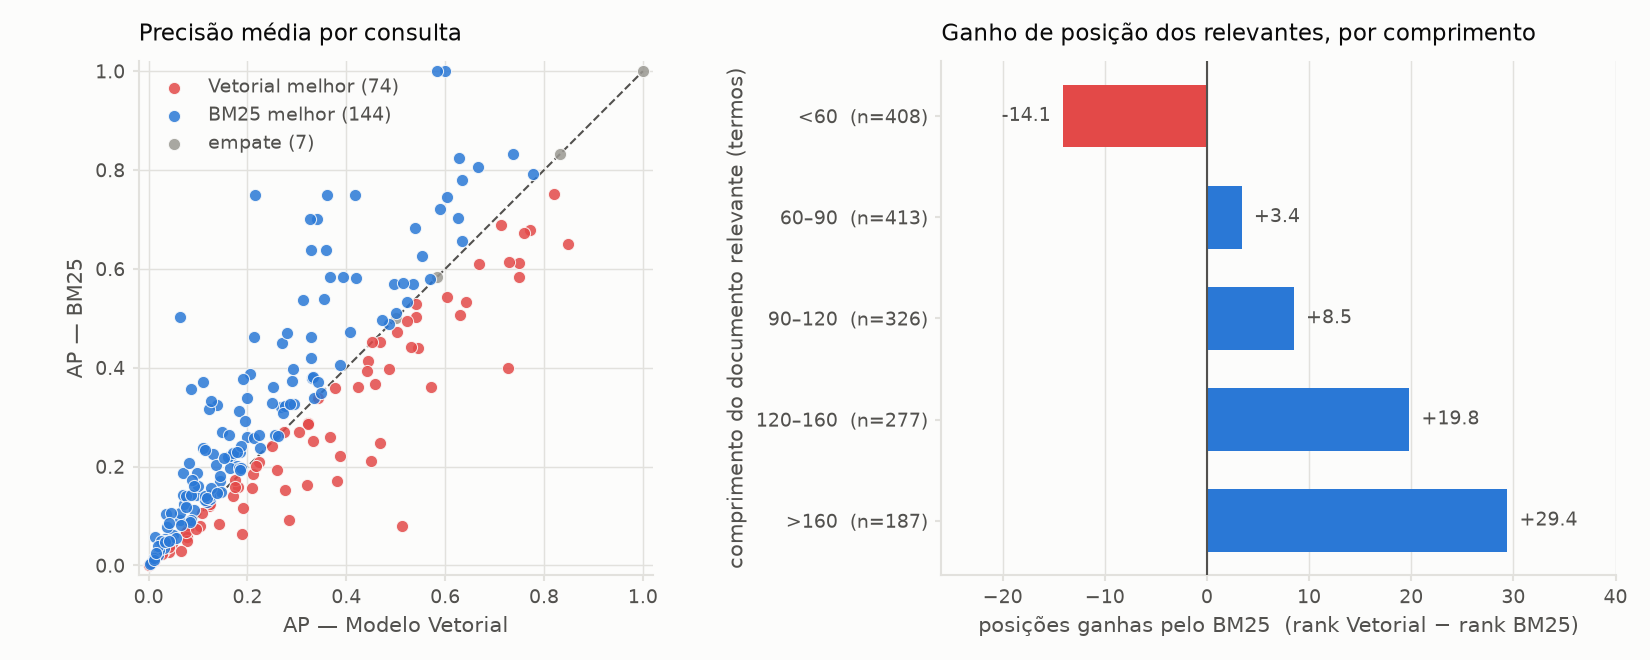
\includegraphics[width=\textwidth]{figuras/comparacao_modelos.png}
\caption{Esquerda: AP de cada consulta nos dois modelos (acima da diagonal, BM25 melhor).
Direita: posições ganhas pelo BM25 para cada par (consulta, documento relevante), por faixa de
comprimento do documento ($\mathrm{avgdl}=94{,}8$).}
\label{fig:comparacao}
\end{figure}

Para entender \emph{onde} ocorrem as diferenças, analisamos
$\Delta\mathrm{AP} = \mathrm{AP}_{\mathrm{BM25}} - \mathrm{AP}_{\mathrm{Vet}}$ por consulta.
Três evidências apontam para o comprimento dos documentos:
\begin{itemize}
  \item \textbf{Correlação com características da consulta.} Das três características testadas,
  só o \textbf{comprimento médio dos documentos relevantes} está associado a $\Delta$AP
  ($r=0{,}374$). O tamanho da consulta ($r=-0{,}067$) e o número de relevantes ($r=-0{,}069$)
  praticamente não têm relação.
  \item \textbf{Ganho de posição por comprimento.} Nos 1612 pares (consulta, documento relevante),
  as posições ganhas pelo BM25 crescem de forma monotônica com o comprimento do documento: o BM25
  \emph{perde} 14,1 posições em documentos com menos de 60 termos e \emph{ganha} 29,4 em
  documentos com mais de 160 (Figura~\ref{fig:comparacao}, direita).
  \item \textbf{Presença no Top-10.} Relevantes com mais de 120 termos aparecem 157 vezes no
  Top-10 do BM25 e 105 no do Vetorial. Com menos de 60 termos a relação se inverte: 128 no BM25
  contra 158 no Vetorial.
\end{itemize}

\textbf{Hipótese: a diferença está na normalização por comprimento.} O cosseno divide o score por
$\lVert\vec d\rVert$, que cresce com \emph{todos} os termos do documento. Assim, um documento
longo é penalizado mesmo quando é longo por tratar o assunto a fundo. No BM25, com $b=0{,}75$, só
75\% do desvio em relação ao avgdl é descontado, e esse desconto age sobre uma tf já saturada, que
não recompensa documentos longos apenas por repetirem termos.

\subsection{Análise por consulta}
As consultas foram escolhidas automaticamente pelo $\Delta$AP, sem seleção manual. A
Tabela~\ref{tab:top5} mostra o Top-5 de cada modelo.

\begin{table}[h]
\centering\footnotesize
\setlength{\tabcolsep}{4pt}
\caption{Top-5 por consulta: \texttt{id}\,(|d|), com relevantes em \textbf{negrito}. A última
coluna traz o comprimento dos relevantes.}
\label{tab:top5}
\begin{tabular}{clcll}
\toprule
Consulta & Modelo & AP & Top-5 & |d| relevantes \\
\midrule
\multirow{2}{*}{167} & Vetorial & 0,216 & 553\,(98) · 1279\,(92) · 1099\,(43) · \R{274}\,(142) · 1100\,(78) & \multirow{2}{*}{142, 195} \\
                     & BM25     & 0,750 & \R{274}\,(142) · 1279\,(92) · 553\,(98) · \R{82}\,(195) · 1098\,(99) & \\
\midrule
\multirow{2}{*}{36}  & Vetorial & 0,064 & 123\,(140) · 281\,(25) · 1299\,(40) · 526\,(71) · 1222\,(120) & \multirow{2}{*}{76, 140} \\
                     & BM25     & 0,503 & \R{168}\,(140) · 123\,(140) · 623\,(118) · 518\,(112) · 959\,(120) & \\
\midrule
\multirow{2}{*}{17}  & Vetorial & 0,513 & \R{106}\,(37) · 336\,(49) · 326\,(33) · 498\,(86) · 1108\,(148) & \multirow{2}{*}{37, 92} \\
                     & BM25     & 0,079 & 1108\,(148) · 1281\,(130) · 336\,(49) · 700\,(69) · 1301\,(93) & \\
\midrule
\multirow{2}{*}{190} & Vetorial & 0,727 & \R{390}\,(75) · \R{391}\,(79) · 1008\,(51) · \R{15}\,(74) · 627\,(85) & \multirow{2}{*}{29, 29, 74, 75, 79} \\
                     & BM25     & 0,399 & \R{390}\,(75) · 627\,(85) · 856\,(142) · \R{15}\,(74) · 1339\,(134) & \\
\midrule
\multirow{2}{*}{13}  & Vetorial & 0,000 & 496\,(69) · 903\,(123) · 520\,(135) · 313\,(34) · 643\,(79) & \multirow{2}{*}{49, 49, 91, 107} \\
                     & BM25     & 0,000 & 496\,(69) · 903\,(123) · 520\,(135) · 313\,(34) · 440\,(57) & \\
\midrule
\multirow{2}{*}{22}  & Vetorial & 0,000 & 153\,(32) · 207\,(101) · 125\,(134) · 254\,(34) · 348\,(98) & \multirow{2}{*}{65} \\
                     & BM25     & 0,000 & 125\,(134) · 560\,(129) · 50\,(98) · 81\,(68) · 413\,(87) & \\
\bottomrule
\end{tabular}
\end{table}

\textbf{(i) BM25 superior: consultas 167 e 36.} Na q167 (\emph{ablative mass loss \ldots\
hypersonic flight}) os dois relevantes têm 142 e 195 termos, bem acima do avgdl. O BM25 coloca o
doc 274 em 1º e o doc 82 em 4º; o Vetorial só alcança o doc 274 na 4ª posição, e seu topo é
ocupado por documentos de 98, 92 e 43 termos, menos penalizados pela divisão pela norma. Na q36 o
efeito é mais forte: o BM25 traz o doc 168 (140 termos) em 1º, enquanto o Vetorial não tem
\emph{nenhum} relevante no Top-5.

\textbf{(ii) Vetorial superior: consultas 17 e 190.} É a situação inversa. O relevante da q17 tem
apenas 37 termos e o Vetorial o põe em 1º; no BM25 ele sai do Top-5, que começa por documentos de
148 e 130 termos e não tem relevante algum. Na q190 os cinco relevantes são curtos (29 a 79 termos), e o
BM25 os troca por documentos de 134 e 142 termos. A \textbf{simetria entre (i) e (ii)} é a
evidência mais forte de que a diferença vem da normalização por comprimento, e não de uma
superioridade genérica de um dos modelos.

\textbf{(iii) Ambos insatisfatórios: consultas 13 e 22.} Das 27 consultas com P@10 $=0$ nos dois
modelos, estas são as duas piores, com AP exatamente 0. O diagnóstico é descasamento de
vocabulário: nenhum documento relevante compartilha \emph{um único termo} com a consulta. Na q13
(\emph{transonic aileron buzz}) os relevantes falam em \emph{shock wave}, \emph{buffeting} e
\emph{vorticity}; na q22, dois termos da consulta (\term{anyon}, \term{els}) sequer existem na
coleção. Com interseção vazia o score é zero por construção, e nenhuma ponderação resolve.

\subsection{Variação dos parâmetros do BM25}\label{sec:param}
\begin{figure}[h]
\centering
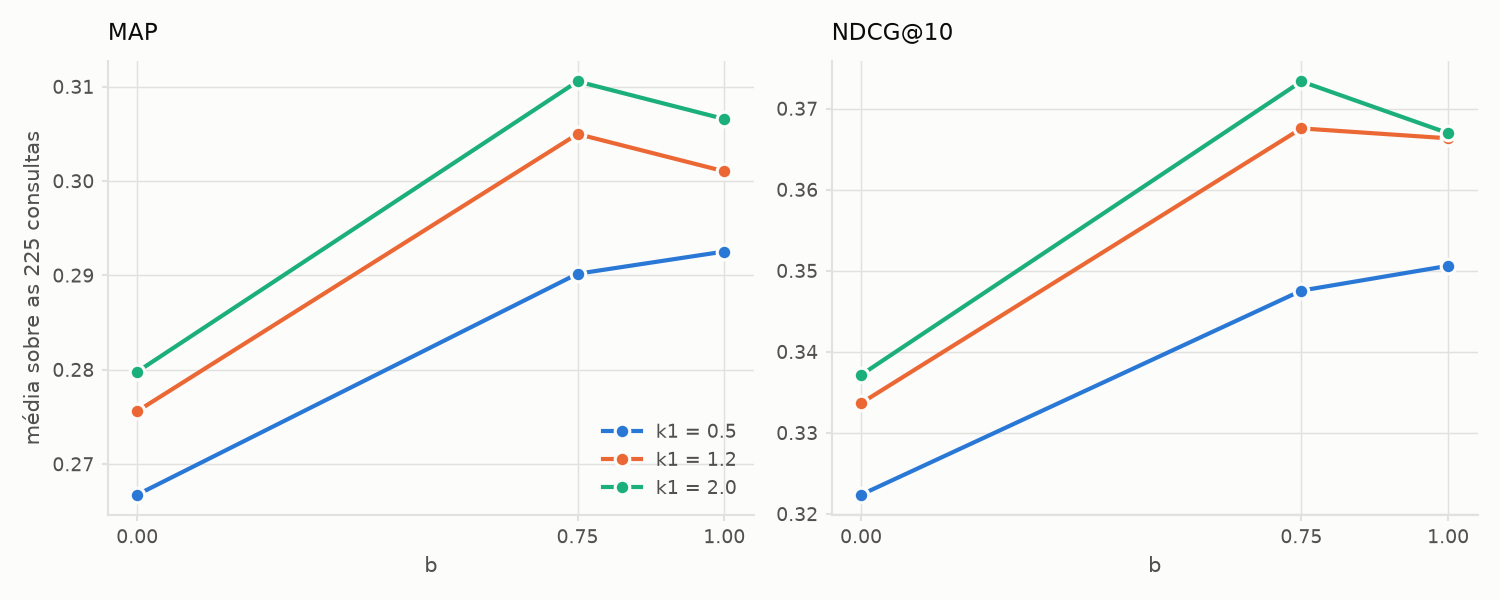
\includegraphics[width=0.82\textwidth]{figuras/grid_bm25.png}
\caption{MAP e NDCG@10 do BM25 (\texttt{stop+stem}) para o grid $k_1\times b$.}
\label{fig:grid}
\end{figure}

\begin{table}[h]
\centering\small
\caption{Grid de parâmetros do BM25: MAP / NDCG@10. Em destaque, o melhor ponto; em itálico, o padrão.}
\label{tab:grid}
\begin{tabular}{cccc}
\toprule
$k_1 \backslash b$ & 0,00 & 0,75 & 1,00 \\
\midrule
0,5 & 0,2668 / 0,3224 & 0,2902 / 0,3475 & 0,2925 / 0,3506 \\
1,2 & 0,2756 / 0,3337 & \emph{0,3050 / 0,3676} & 0,3010 / 0,3663 \\
2,0 & 0,2798 / 0,3371 & \textbf{0,3106 / 0,3734} & 0,3066 / 0,3670 \\
\bottomrule
\end{tabular}
\end{table}

A Figura~\ref{fig:grid} e a Tabela~\ref{tab:grid} mostram que as duas métricas
concordam: o melhor ponto é $k_1=2{,}0$, $b=0{,}75$ em ambas, e a ordenação das nove células é
praticamente a mesma.
\begin{itemize}
  \item $b$ tem mais efeito que $k_1$: passar $b$ de 0 para 0,75 (com $k_1=1{,}2$) rende
  +10,7\% de MAP; variar $k_1$ de 0,5 para 2,0 (com $b=0{,}75$) rende +7,0\%.
  \item $b=0$ é a única escolha claramente ruim. De 0 para 0,75 o ganho é grande; de 0,75
  para 1 há uma leve \emph{perda} (exceto com $k_1=0{,}5$). Alguma normalização por comprimento é
  essencial, mas a normalização total é excessiva, o que é coerente com a Seção 4.2: o Vetorial,
  que sempre normaliza pela norma completa, perde justamente nos documentos longos.
  \item $k_1=2{,}0$ vence nas três colunas. Saturar mais devagar favorece esta coleção de
  resumos técnicos curtos, nos quais repetir um termo indica o assunto do texto, e não
  enchimento.
  \item O melhor ponto rende apenas +1,8\% sobre o padrão; mantivemos $k_1=1{,}2$ e
  $b=0{,}75$ nos demais experimentos.
\end{itemize}

\textbf{Consulta em que $b$ muda o ranking: q161} (\emph{integral method \ldots\ laminar separation
point}). Entre $b=0$ e $b=1$ só 3 dos 10 primeiros documentos são comuns. Com $b=0$, os
documentos 329, 962 e 364 (376, 232 e 214 termos, nenhum relevante) ocupam as posições 3 a 5,
e o Top-5 tem em média 218 termos. Com $b=0{,}75$ ou 1 eles saem, o comprimento médio do Top-5 cai
para 95 termos ($\approx$ avgdl), o relevante doc 55 (81 termos) entra em 3º e o AP@10 sobe de
0,417 para 0,500. Isso confirma, \emph{manipulando o parâmetro}, o que as Seções 4.2 e 4.3
observaram.

\subsection{Modificação de consultas}
Reformulamos cinco consultas a partir do texto da consulta e de conhecimento de domínio e
executamos as versões original e modificada nos dois modelos (Tabela~\ref{tab:reform}).

\begin{table}[h]
\centering\footnotesize
\setlength{\tabcolsep}{3.5pt}
\caption{Reformulações (\texttt{stop+stem}). Métricas no formato original $\to$ modificada;
``troc.'' = documentos trocados no Top-10 (Vetorial / BM25).}
\label{tab:reform}
\begin{tabular}{c>{\raggedright\arraybackslash}p{5.6cm}cccccc}
\toprule
\multirow{2}{*}{Q} & \multirow{2}{*}{Consulta modificada (tipo)} & \multicolumn{2}{c}{P@10} & \multicolumn{2}{c}{NDCG@10} & \multirow{2}{*}{troc.} \\
\cmidrule(lr){3-4}\cmidrule(lr){5-6}
 & & Vetorial & BM25 & Vetorial & BM25 & \\
\midrule
22  & \emph{turbulent skin friction viscosity variation with temperature} (remoção de termos não-conteúdo)
    & 0,0 $\to$ 0,0 & 0,0 $\to$ 0,0 & 0,000 $\to$ 0,000 & 0,000 $\to$ 0,000 & 3 / 1 \\
13  & \emph{transonic aileron buzz shock wave boundary layer interaction control surface oscillation} (acréscimo)
    & 0,0 $\to$ \textbf{0,1} & 0,0 $\to$ \textbf{0,1} & 0,000 $\to$ \textbf{0,184} & 0,000 $\to$ \textbf{0,199} & 6 / 7 \\
82  & \emph{methods for calculating lift distribution on swept wings in subsonic flow} (remoção de nomes próprios)
    & 0,2 $\to$ 0,2 & 0,3 $\to$ 0,2 & 0,517 $\to$ 0,517 & 0,540 $\to$ \textbf{0,275} & 2 / 3 \\
200 & \emph{buckling stresses in torispherical shells} (mais genérica)
    & 0,1 $\to$ 0,1 & 0,2 $\to$ 0,1 & 0,235 $\to$ 0,296 & 0,370 $\to$ 0,296 & 6 / 6 \\
95  & \emph{theoretical heat transfer distribution around a hemisphere blunt nosed body stagnation point} (mais específica)
    & 0,1 $\to$ 0,1 & 0,2 $\to$ 0,2 & 0,065 $\to$ \textbf{0,272} & 0,416 $\to$ 0,411 & 6 / 4 \\
\bottomrule
\end{tabular}
\end{table}

\textbf{Reformular muda muito o ranking, mas o efeito médio é pequeno e instável.} Em média 4,4
dos 10 documentos do Top-10 são trocados. O P@10 médio fica igual (0,110 $\to$ 0,110) por
compensação: a q13 ganha um relevante nos dois modelos, enquanto o BM25 perde um na q82 e outro
na q200. O NDCG@10 médio sobe de 0,214 para 0,245, mas o ganho vem quase todo de dois casos: a
q13, que passa a recuperar um relevante, e o Vetorial na q95; sem eles, a média cairia. Dos 10
casos, 4 melhoram, 3 pioram e 3 ficam iguais em NDCG@10: é uma intervenção de alta variância, cujo
efeito depende da consulta e do modelo. A dependência do modelo é clara: generalizar a q200
melhora o Vetorial e piora o BM25, e especificar a q95 melhora muito o Vetorial
(0,065 $\to$ 0,272) e deixa o BM25 praticamente parado. A reformulação manual interage com o
modelo e não é uma melhoria independente dele.
\begin{itemize}
  \item \textbf{q13 sai do zero.} O acréscimo de \emph{shock wave}, \emph{boundary layer} e
  \emph{interaction} cria a interseção que faltava, e o relevante doc 265 entra no Top-10 dos dois
  modelos (5º no BM25). Isso confirma na prática o diagnóstico da Seção 4.3: quando a falha é de
  vocabulário, só mudar a representação da consulta resolve. Mas a expansão também trouxe dois
  documentos vizinhos não relevantes (335 e 798, sobre interação choque-camada limite).
  \emph{Ressalva:} os termos acrescentados se justificam pela física (o \emph{buzz} transônico é
  causado pela interação entre onda de choque e camada limite), mas coincidem com o vocabulário que
  o diagnóstico da Seção 4.3 encontrou nos relevantes. Por isso, este ganho não é uma evidência
  independente dos qrels.
  \item \textbf{q22 continua em zero.} Retirar os termos conversacionais eliminou ruído, mas não
  \emph{acrescentou} nenhum termo do relevante. Remover ruído não é o mesmo que expandir o
  vocabulário.
  \item \textbf{q82 é o fracasso instrutivo.} Remover os nomes de autores derrubou o NDCG@10 do
  BM25 de 0,540 para 0,275. O termo \term{kuchemann} tem df $=1$ (idf $=6{,}84$) e apontava
  exatamente para o artigo relevante 678, que cai de 1º para 3º (\emph{multhopp} nem existe na
  coleção). O que parecia ruído era o sinal mais forte da consulta.
\end{itemize}

\subsection{Análise de erros}
Os casos foram selecionados por critério programático sobre o BM25 (\texttt{stop+stem}): para os
não relevantes no topo, documentos de grau $-1$ em 1º lugar; para o relevante fora do Top-10, o
documento de grau 1 (resposta completa, a falha mais grave possível) com a pior posição.

\textbf{Não relevante em 1º -- q7, doc 492 (score 64,08, o maior entre os erros desse tipo).} A
consulta pede \emph{pressure distributions for an ogive forebody at angle of attack}; o título do
documento é \emph{prediction of ogive-forebody pressures at angles of attack}. A decomposição do
score mostra por que ele é tão alto: dois termos raríssimos, \term{ogiv} (df $=14$, idf $=4{,}57$,
contribuição 15,3) e \term{forebodi} (df $=8$, idf $=5{,}10$, contribuição 17,1), \emph{somados} a
tf $=4$ em \term{pressur}, \term{angl} e \term{attack} num documento curto de 34 termos, que o fator
$b$ favorece. Alto idf e alta tf ao mesmo tempo, e mesmo assim o documento é julgado com grau $-1$.

\textbf{Não relevante em 1º -- q13, doc 496, nos dois modelos.} O termo \term{buzz} tem df $=1$ e
idf $=6{,}84$: existe em um único documento da coleção, justamente este (\emph{a theory of
transonic aileron buzz}), e sozinho garante a primeira posição. Também é julgado com grau $-1$.

\textbf{O padrão por trás dos dois casos.} Cada consulta tem exatamente um documento de grau
$-1$, e ele fica sistematicamente no topo: em 1º lugar em 96 das 225 consultas no BM25 (43\%) e
em 81 no Vetorial (36\%); no Top-10 em 72\% e 69\%, respectivamente (posição mediana 2 e 3). Há
também indícios estruturais: o id desse documento tem correlação de 0,662 com o número da consulta,
e consultas consecutivas compartilham o mesmo documento (q1/q2 $\to$ 486, q7/q8 $\to$ 492,
q13/q14 $\to$ 496). A explicação mais provável é que o documento de grau $-1$ seja o
artigo a partir do qual a consulta foi formulada. Isso explica o casamento lexical quase
perfeito e a numeração correlacionada, e o julgamento ``\emph{references of no interest}'' faz
sentido para quem já conhece o artigo. Consequência: em 43\% das consultas o melhor resultado do
BM25 conta como erro \emph{por construção da coleção}, o que impõe um teto à P@10 que não vem de
falha de modelagem.

\textbf{Relevante fora do Top-10 -- q176, doc 583 (grau 1, posição 939 de $\sim$1400).} A
consulta é \emph{some approximate analytical heat conduction solutions using methods other than
biot's principle}; o documento, \emph{influence coefficients for real gases}, é julgado como
resposta completa. Dos 9 termos da consulta ele compartilha só um: \term{use}, um verbo genérico
(idf $=1{,}00$), sem poder discriminativo. É o oposto dos casos anteriores: casamento lexical
quase nulo e relevância máxima. O julgamento se apoia no conteúdo conceitual do artigo, não no
vocabulário, e nenhum modelo baseado em sobreposição de termos consegue recuperá-lo.

% ==================================================================
\section{Considerações Finais}
% ==================================================================
\begin{enumerate}
  \item \textbf{A normalização por comprimento é o que separa os dois modelos.} A correlação com
  $\Delta$AP ($r=0{,}374$), o ganho por faixa de comprimento (+29,4 posições para relevantes
  longos), a simetria dos casos individuais e o experimento com $b$ apontam para a mesma causa. O
  Modelo Vetorial é um extremo rígido dessa escala: normaliza sempre pela norma completa, sem um
  parâmetro que possa relaxar a normalização.
  \item \textbf{O descasamento de vocabulário é o teto dos dois modelos.} Ambos pontuam por
  sobreposição ponderada de termos; com interseção vazia o score é zero, e nenhum ajuste de
  ponderação, $k_1$ ou $b$ muda isso. Só mudar a representação da consulta funciona, e mesmo assim
  de forma imprecisa (q13). O caminho robusto seria uma representação semântica (expansão de
  consulta, embeddings).
  \item \textbf{Termos de df muito baixo são apostas de alto risco.} O idf os torna decisivos nos
  dois sentidos: \term{kuchemann} (df $=1$) era o melhor sinal da q82, e \term{buzz} (df $=1$)
  sozinho pôs um não relevante em 1º na q13.
  \item \textbf{Hierarquia dos ganhos de MAP}: pré-processamento (\texttt{nada} $\to$
  \texttt{stop+stem}, BM25) \textbf{+13,2\%}; modelo (Vetorial $\to$ BM25, \texttt{stop+stem})
  \textbf{+12,2\%}; ajuste de parâmetros do BM25 (padrão $\to$ melhor ponto) +1,8\%. Pré-processamento
  e escolha do modelo valem uma ordem de grandeza a mais que o ajuste fino, e os valores
  convencionais $k_1=1{,}2$, $b=0{,}75$ já são adequados para esta coleção.
\end{enumerate}

% ==================================================================
\section{Uso de ferramentas de IA}
% ==================================================================
% TODO: revisar/completar conforme o uso real do grupo durante a implementação.
Utilizamos o assistente Claude (Anthropic) como apoio na redação e formatação deste relatório em
Latex, a partir dos resultados e das análises produzidos pelo grupo no notebook. Em relação ao código do projeto, utilizamos a IA para auxiliar a escrever algumas partes do código que estávamos em dúvida, a depurar o código e na revisão de respostas.

\end{document}
